\chapter{Análise de Resultados}
Neste capítulo, os resultados obtidos com a execução dos \textit{profiles} de falhas Moderado e Intenso, que foram apresentadas na Seção 4.3, são executados e analisados. Busca-se concluir que há otimização das métricas de desempenho de escalonamento no escalonador proposto em comparação com as abordagens padrão do \textit{Kubernetes} (com e sem réplica) em cenários de falhas. Na Seção 5.1 serão apresentados os resultados para base de comparação, em sequência, nas Seções 5.2 e 5.3 os resultados com interferência das falhas de escalonamento. Para cada análise de cenário, será apresentada uma tabela que representa a média dos valores encontrados nos testes, enquanto os gráficos temporais são baseados na mediana. Além disso, o escalonador padrão será denominado \textit{Padrão}, e a configuração com réplicas de \textit{Padrão*}. O escalonador proposto é denominado de \textit{KMS}. Ao fim do capítulo será feita uma revisão e conclusão dos testes realizados.

\section{Cenário referência}

Esse cenário investigou os valores usados como base de comparação para as métricas de escalonamento sem a interferência de falhas. Portanto, é considerado o valor referência da análise, pois evidenciará a perda de desempenho do escalonamento ao ser comparado com os \textit{profiles} das seções posteriores.

A Figura \ref{fig:cenario-base} representa a composição dos resultados. Na tabela são informadas as médias dos testes executados para cada abordagem de escalonamento, já os gráficos mostram a média cumulativa da métrica analisada. Nos gráficos notou-se que os resultados do \ac{KMS} degradaram em relação as outras abordagens no momento em que é submetida a uma carga maior de escalonamento (segundo 90 em diante). Isso deve-se a sobrecarga da arquitetura baseada em microsserviços, principalmente influenciada pelas trocas de mensagens entre os sistemas. Outro fator a salientar, o \textit{KMS} faz requisições ao \textit{Kube-API} para buscar a lista de \textit{Pods} e enviar ordens de escalonamento, logo está submetido ao tempo de resolução desse serviço. O \textit{Kube-Scheduler} também utiliza a \textit{Kube-API}, entretanto, possui maior prioridade por se tratar de um serviço do \textit{Control Plane}.

 \begin{figure}[!ht]
	\centering
	\begin{tabular}[b]{cccc}\hline
		Escalonador & Tempo Espera & \textit{Makespan} & \textit{Slowdown}\\ \hline
		Padrão  & 2,765s & 38,551s & 1,702\\
		Padrão* & 3,70s  & 43,636s & 1,166 \\
		KMS     & 4,49s & 41,789s & 1,860 \\ \hline
	\end{tabular}
	\qquad
	\subfloat[\centering Média cumulativa do Tempo de espera]{{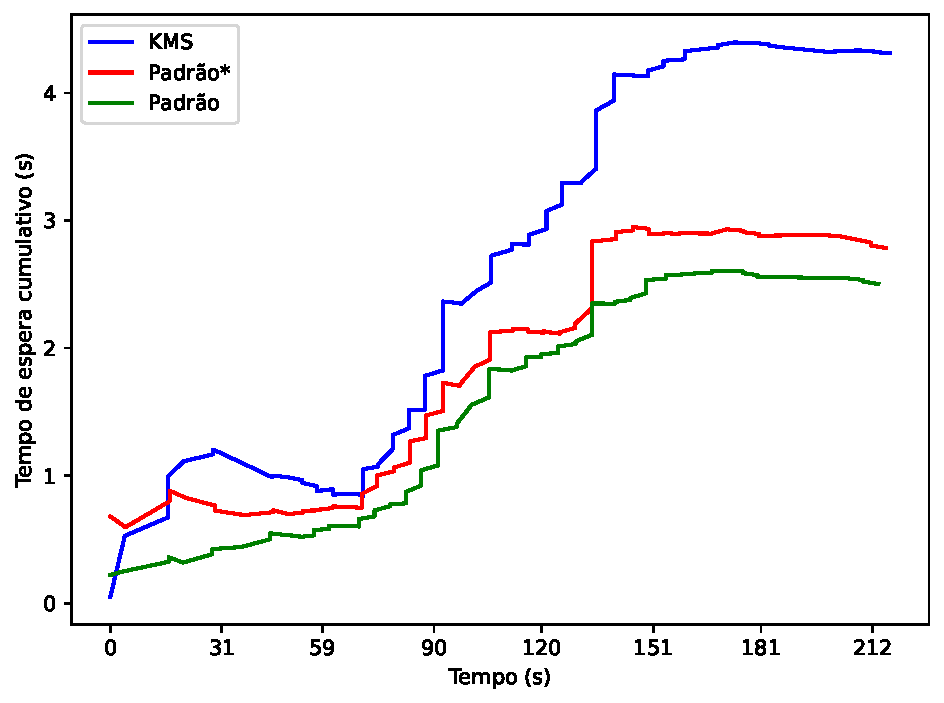
\includegraphics[width=.465\linewidth]{assets/waittime-base.pdf} }}
	\qquad
	\subfloat[\centering Média cumulativa do Makespan]{{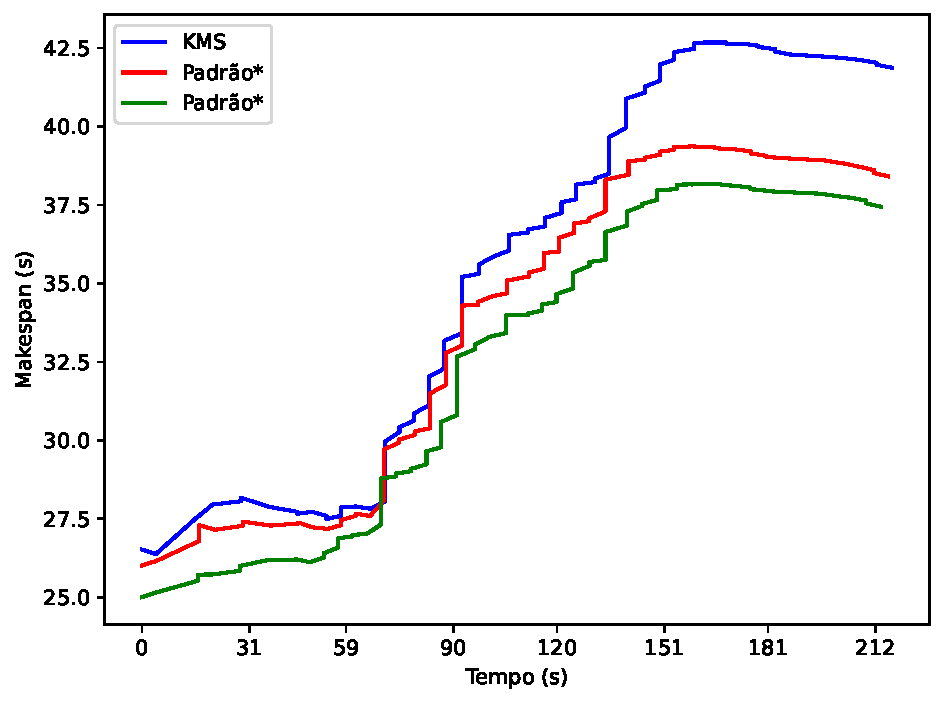
\includegraphics[width=.465\linewidth]{assets/makespan-base.pdf} }}
	\qquad
	\subfloat[\centering Média cumulativa do Slowdown]{{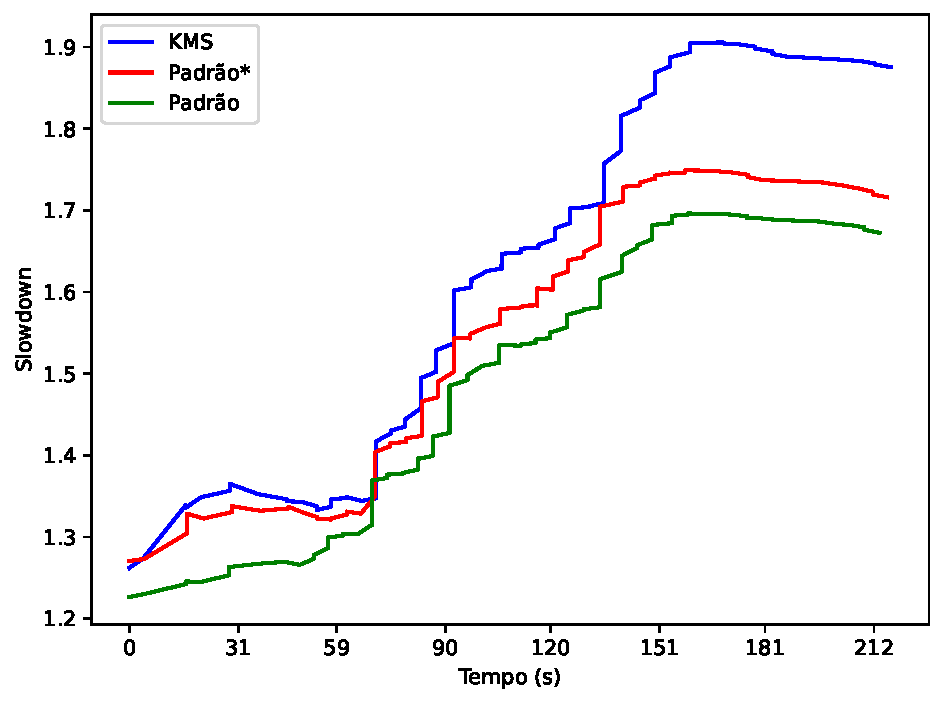
\includegraphics[width=.57\linewidth]{assets/slowdown-base.pdf} }}
	\caption{Composição resultados Referência: Tabela e gráficos de desempenho}
	\label{fig:cenario-base}
\end{figure}

Os gráficos evidenciaram, de forma geral, uma proporção entre os resultados. Esse comportamento era o esperado no cenário base pois não houveram interferência de falhas nem sobrecarga dos recursos computacionais do \textit{cluster}. Nota-se os resultados positivos que a abordagem Padrão apresentou no Tempo de Espera, já o escalonador com réplica resultou em uma ótima taxa de \textit{Slowdown}, evidenciando melhor equilíbrio entre o tempo de espera e escalonamento das cargas de trabalho.


 \newpage
\section{Resultados para o cenário Moderado}
O plano de testes moderado consistiu em submeter os escalonadores às falhas de escalonamento. No total foram 6 simulações de \textit{crashes}, com o objetivo de comprovar que o escalonador padrão degrada as métricas de desempenho, enquanto que o escalonador com réplica e o \textit{KMS} possuem um melhor controle perante falhas.

\begin{figure}[!ht]
	\centering
	\begin{tabular}[b]{cccc}\hline
		Escalonador & Tempo Espera & \textit{Makespan} & \textit{Slowdown}\\ \hline
		Padrão  & 24,84s & 69,57s & 3,13\\
		Padrão* & 8,62s  & 49,71s & 2,178 \\
		KMS     & 4,87s & 43,22s & 1,92 \\ \hline
	\end{tabular}
	\qquad
	\subfloat[\centering Média cumulativa do Tempo de espera]{{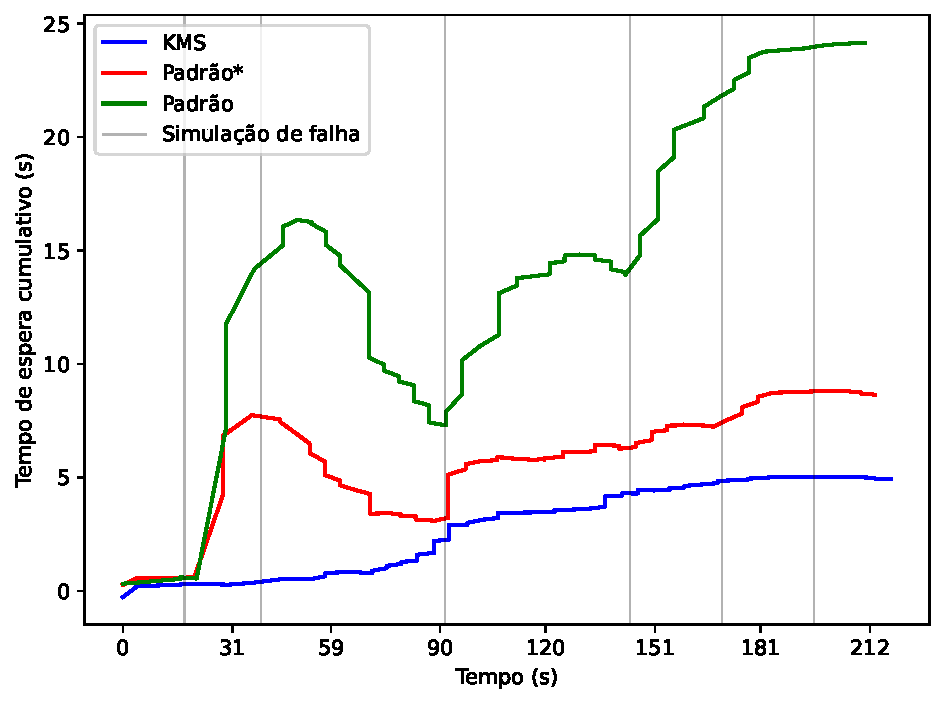
\includegraphics[width=.465\linewidth]{assets/waittime-moderado.pdf} }}
	\qquad
	\subfloat[\centering Média cumulativa do Makespan]{{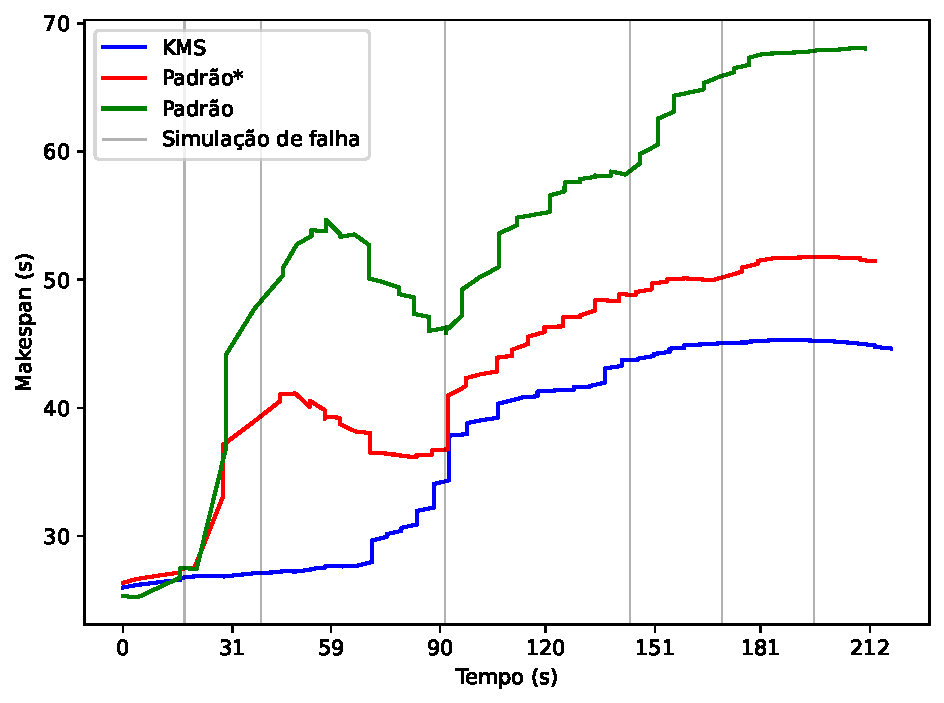
\includegraphics[width=.465\linewidth]{assets/makespan-moderado.pdf} }}
	\qquad
	\subfloat[\centering Média cumulativa do Slowdown]{{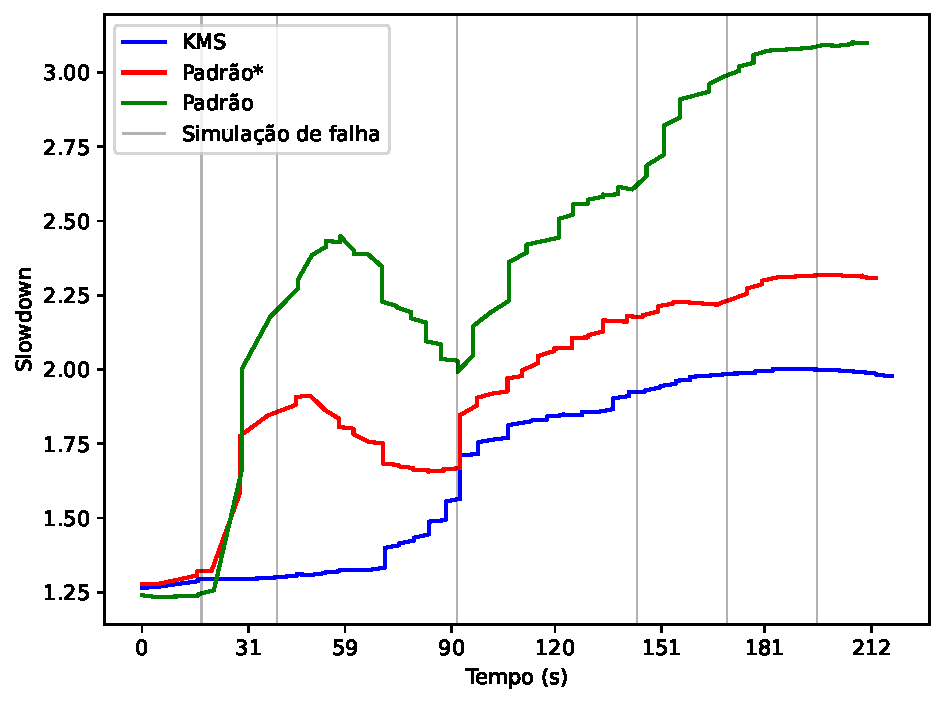
\includegraphics[width=.57\linewidth]{assets/slowdown-moderado.pdf} }}
	\caption{Composição resultados Moderado: Tabela e gráficos de desempenho}
	\label{fig:cenario-base}
\end{figure}

%Neste \textit{profile} obteve-se resultado acima do esperado com o \textit{KMS}, pois o número de falhas era consideravelmente pequeno, entretanto, foi o suficiente para degradar as métricas do escalonador \textit{Padrão} e o \textit{Padrão*}.
Neste \textit{profile} é possível analisar a queda de desempenho das abordagens quando são injetados erros de escalonamento. Embora exista degradação em todas as comparações, como é visto no escalonador \textit{Padrão} que piorou a métrica de tempo de espera em 798\% e o \textit{Padrão*} em 132\%, o \textit{KMS} degradou a métrica de tempo de espera em apenas 8\%. Os dois primeiros são sistemas monolíticos que possuem dependências e inicializações complexas, acarretando em deixar o processo de escalonamento ocioso por certos períodos de tempos. Por sua vez, o \textit{KMS}, quando ocorre alguma falha, apenas uma instância do sistema é derrubada e todas as outras estão ativas resolvendo escalonamento. As falhas no \textit{KMS} influenciaram pouco em comparação com o teste anterior, houve uma variação de apenas 0,38s no tempo de espera, 1,43s de \textit{makespan} e 0,06 de \textit{slowdown}. Nos intervalos [0,90] dos gráficos, nota-se um pico de aumento nas métricas. O escalonador padrão com réplica suportou bem esse pico, isso é evidenciado no tempo 90 em que igualou suas médias cumulativas das métricas com o \ac{KMS}. Entretanto, no decorrer dos testes, foram simuladas mais falhas distanciando as métricas das abordagens apontando o desempenho do \ac{KMS}.

\newpage
\section{Resultados para o cenário Intenso}
Para o \textit{profile} Intenso,  foi configurado uma elevada taxa de falhas durante o período de testes, aumentando o tempo de indisponibilidade do escalonador \textit{Padrão}. Por esse motivo foram desconsiderados os valores dessa abordagem, e a análise considera somente as métricas de escalonamento do \textit{Padrão*} e \textit{KMS}.

\begin{figure}[!ht]
	\centering
	\begin{tabular}[b]{cccc}\hline
		Escalonador & Tempo Espera & \textit{Makespan} & \textit{Slowdown}\\ \hline
		Padrão  & N/C & N/C & N/C\\
		Padrão* & 29,83s  & 78,62s & 3,52 \\
		KMS     & 10,52s & 52,59s & 1,92 \\ \hline
	\end{tabular}
	\qquad
	\subfloat[\centering Média cumulativa do Tempo de espera]{{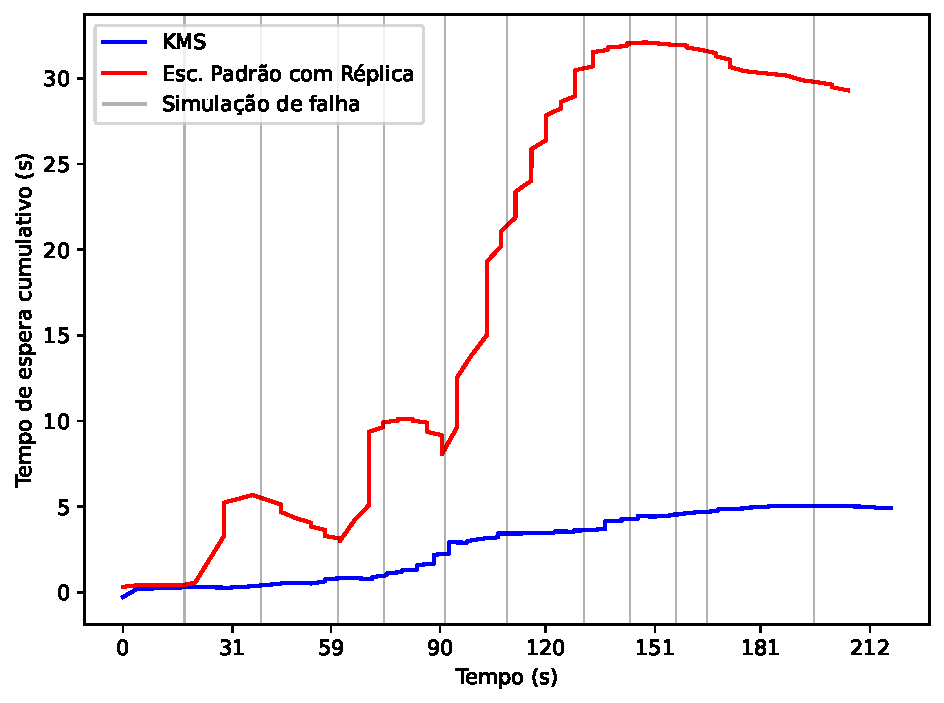
\includegraphics[width=.465\linewidth]{assets/waittime-intenso.pdf} }}
	\qquad
	\subfloat[\centering Média cumulativa do Makespan]{{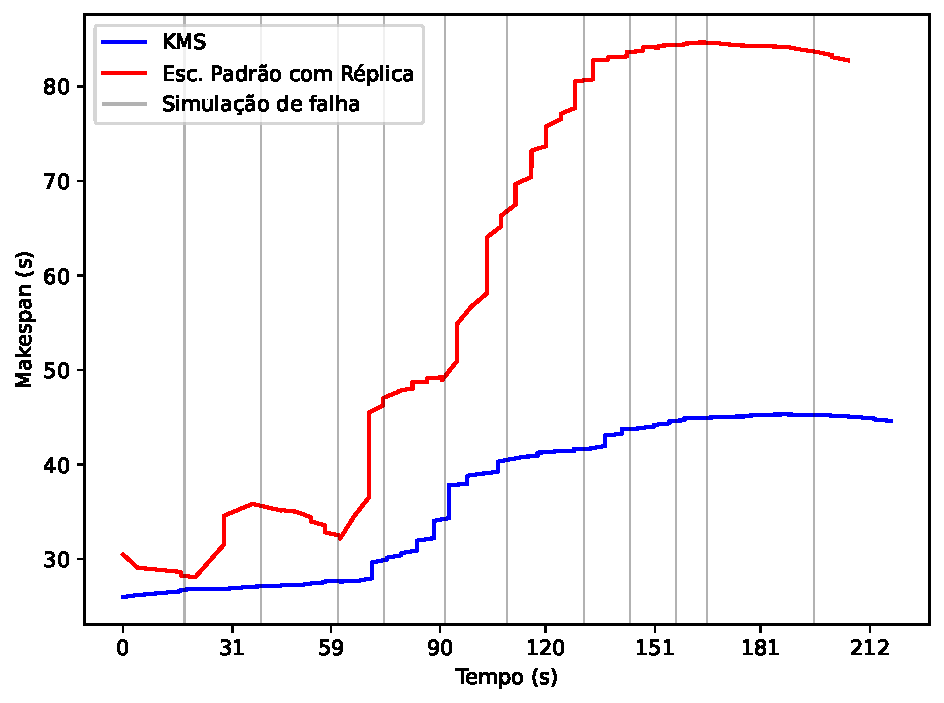
\includegraphics[width=.465\linewidth]{assets/makespan-intenso.pdf} }}
	\qquad
	\subfloat[\centering Média cumulativa do Slowdown]{{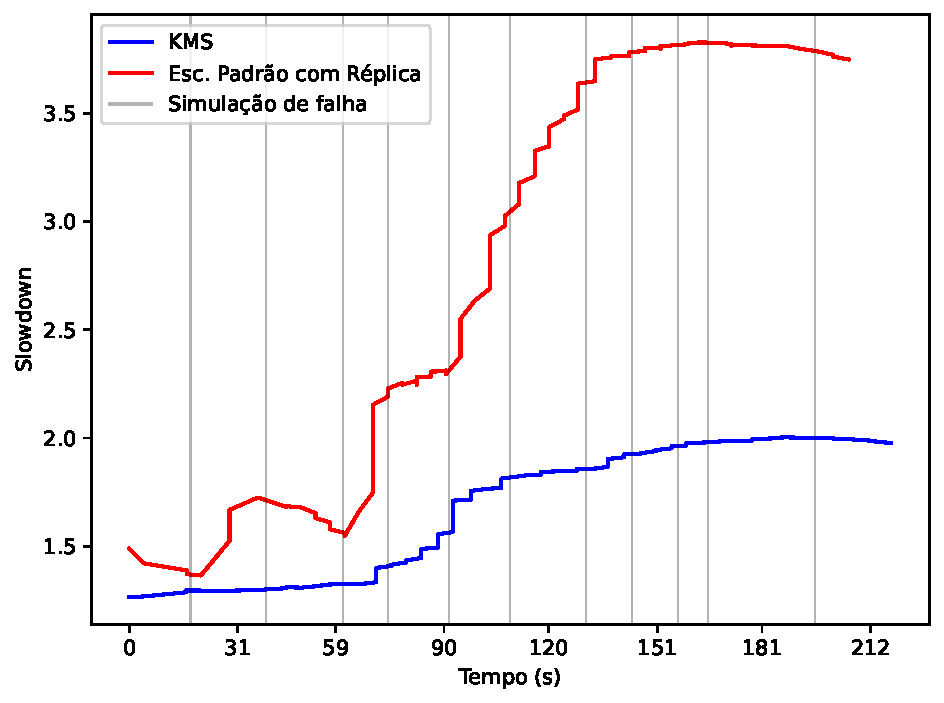
\includegraphics[width=.57\linewidth]{assets/slowdown-intenso.pdf} }}
	\caption{Composição resultados Intenso: Tabela e gráficos de desempenho}
	\label{fig:cenario-intenso}
\end{figure}

O \textit{Profile} Intenso foi desenvolvido para apontar o desempenho do \textit{KMS} quando é submetido a um grande volume de falhas em sequência. A abordagem de réplica do \textit{Kubernetes} é interessante e possui uma ótimo desempenho em cenários moderados, entretanto, em um cenário caótico as métricas são degradadas como comprovam os gráficos da Figura \ref{fig:cenario-intenso}. Possuindo um pico acentuado a partir do tempo 90, enquanto que o \textit{KMS} possui um pico controlado, devido as suas características de sistemas distribuídos e microsserviços.

\section{Considerações parciais}
Os testes executados demonstraram a eficiência do escalonador proposto \ac{KMS} em cenários de falhas. A abordagem \textit{Padrão} do \textit{Kubernetes} foi bem avaliada no cenário referência, enquanto nos cenários Moderado e Intenso, ocorreram degradações consideráveis nas suas métricas de desempenho. Por fim, a abordagem \textit{Padrão*} desempenhou bem no cenário Moderado, evidenciando o ganho de desempenho ao utilizar alta disponibilidade de escalonamento. Já no cenário Intenso, o elevado volume de submissões de falhas nos hospedeiros dos escalonadores resultou no agravamento nos valores das métricas avaliadas.

A Seção 5.1 apontou os valores bases das métricas de escalonamento em um cenário sem falhas. Nesse contexto, o escalonador padrão do \textit{Kubernetes} obteve os melhores resultados em comparação com as outras técnicas abordadas. Essa diferença deve-se a sobrecarga que sistemas distribuídos possuem, principalmente em comunicação. Na seção seguinte, evidenciou-se que um tratamento de falhas é ideal para a disponibilidade do serviço de escalonamento, pois o escalonador proposto possui um desempenho superior em comparação ao escalonador padrão. Por fim, na execução dos testes no cenário Intenso, as métricas de escalonamento foram concebíveis apenas na execução do \textit{KMS}, expondo que um sistema distribuído baseado em microsserviços possui um desempenho não alcançado pelos escalonadores monolíticos.




















